\subsection{Comparison of Displayed Summary with Hidden Reasoning}
\label{app:summary}

Claude's extended-thinking API returns only a short \emph{summary} of the
model's reasoning to the user (\texttt{display: summarized}), rather than
the full chain of thought. OpenAI's Responses API does the same. The user only sees the output of a separate
summarizer (\texttt{summary: auto}). \Cref{fig:summary_vs_thinking} compares summary length with the
length of the hidden reasoning trace for different Claude models. By contrast, the signature
reconstruction in \Cref{fig:teaser} recovers nearly the entire trace.
Decoding the signature therefore reveals approximately five times more
reasoning than the provider exposes through the summary.

\begin{figure}[h]
\centering
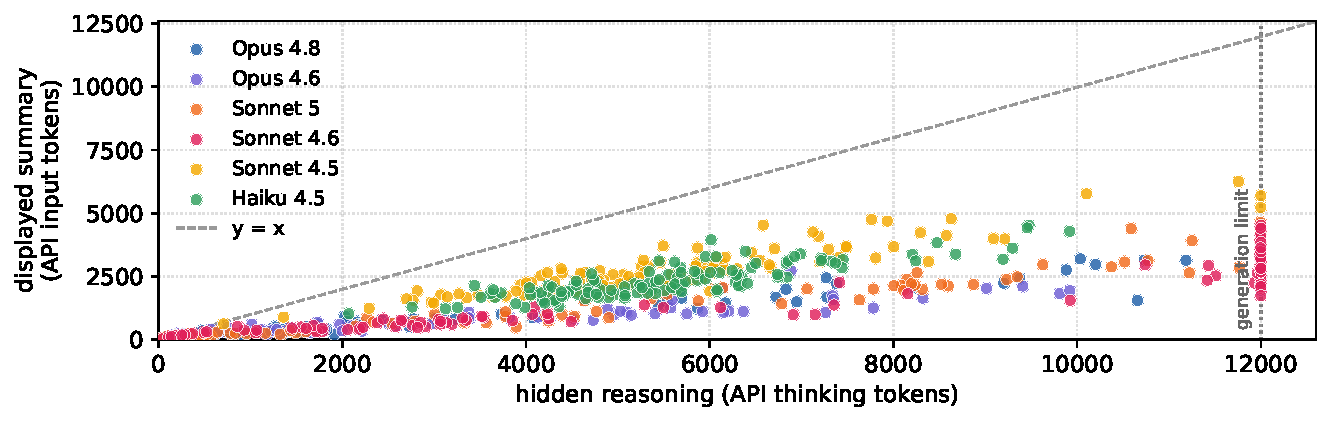
\includegraphics[width=\linewidth]{figures/faithfulness/summary_vs_thinking.pdf}
\caption{\textbf{The displayed summary is a small fraction of the hidden reasoning.}
For each Codeforces problem, the hidden thinking tokens the source model generated
(reported by the API, $x$) versus the token length of the displayed summary
($y$).}
\label{fig:summary_vs_thinking}
\end{figure}


\paragraph{Summarization Effects.}
The reasoning summary is a condensed version of the raw reasoning, typically produced by a cheaper, less capable model and made available to users through the API. We study the effects of this summarization process and the artifacts it may introduce. We decode hidden reasoning traces on AIME~2025 and retain only those whose decoded length matches the API-reported hidden-trace length within $5\%$. This yields a small dataset of 18 Opus~4.8 traces and 15 GPT-5.6-Sol traces, with one sample per problem. We use an LLM judge and Claude Code to surface candidate cases, and manually inspect every summary--reasoning pair.

In 9 of the 18 Opus traces, the hidden reasoning states the answer before deriving it. In 8 of these cases, the summary also reports the answer in advance. In the remaining case, the difference hinges on a single phrase: ``Let me verify by computing'' becomes ``Let me set up coordinates'' (\Cref{fig:sf_verify_cue}). The surrounding computation is otherwise unchanged, causing the summary to present a verification as if it were an independent derivation.

In another example, a hedged recollection is presented in the summary as a definite value, two sentences before the reasoning correctly computes it (\Cref{fig:sf_fabricated_fact}). A further summary captures only the closing portion of the reasoning, which concerns answer formatting and contains no mathematical content (\Cref{fig:sf_sol_meta}). These artifacts are consistent with a less capable model summarizing reasoning produced by a more capable model.
% Summarization-effect exhibits: decoded reasoning vs. the summary returned
% by the API. Examples 1-2: Opus 4.8. Examples 3-4: GPT-5.6-sol.
% Uses the panel machinery defined in
% sections/92_traces_analysis/03_output_style_drift.tex (promptrow, reasoncol,
% \plabel, \hlseed, \elide) — \input after those definitions.

% ---------------------------------------------------------------------------
% Example 1 — a hedge is lost in compression (Opus 4.8, 2025-I-12)
% ---------------------------------------------------------------------------
\begin{figure}[H]
\centering
\setlength{\columnsep}{12pt}
\setlength{\colw}{\dimexpr(\linewidth-\columnsep)/2\relax}
\begin{promptrow}
\caret\plabel{Prompt}\par\vspace{4pt}
The set of points in \$3\$-dimensional coordinate space that lie in the plane \$x+y+z=75\$ whose coordinates satisfy the inequalities \$x-yz<y-zx<z-xy\$ forms three disjoint convex regions. Exactly one of those regions has finite area. The area of this finite region can be expressed in the form \$a\textbackslash{}sqrt\{b\}\$, where \$a\$ and \$b\$ are positive integers and \$b\$ is not divisible by the square of any prime. Find \$a+b.\$
\end{promptrow}
\vspace{12pt}
\noindent
\begin{reasoncol}[equal height group=sfB]
  \caret\plabel{Reasoning summary (returned by API)}\par\vspace{4pt}
  \raggedright
  I'm verifying the answer by working through the inequalities. The conditions \(x-yz<y-zx<z-xy\) simplify to \((x-y)(1+z)<0\) and \((y-z)(1+x)<0\), and with the constraint \(x+y+z=75\), \hlseed{the finite region has area 225 with a+b = 510.} So the conditions simplify to \(x>-1\), \(x<y\), and \(y<(75-x)/2\), which gives me a bounded region. With \(x\) constrained to \((-1,25)\), I can now find the vertices by looking at where these boundary lines intersect.\par\vspace{3pt}
  The three boundaries are \(x=-1\), \(x=y\), and \(x+2y=75\). Their pairwise intersections give me three vertices: A at \((-1,-1,77)\), B at \((-1,38,38)\), and C at \((25,25,25)\). Now I'm computing the area of this triangle using the cross product of vectors AB and AC.\par\vspace{3pt}
  The cross product works out to \((-1014,-1014,-1014)\), which has magnitude \(1014\sqrt3\), giving an area of \(507\sqrt3\). So \(a=507\) and \(b=3\), making \(a+b=510\).
\end{reasoncol}\hspace{\columnsep}%
\begin{reasoncol}[equal height group=sfB]
  \caret\plabel{Decoded reasoning}\par\vspace{4pt}
  \raggedright
  \hlseed{Answer is 510.}\par\vspace{2pt}
  Let me verify. The inequalities: \(x-yz < y-zx < z-xy\).\par
  First: \(x-yz < y-zx \Rightarrow x-y+zx-yz<0 \Rightarrow (x-y)+z(x-y)<0 \Rightarrow (x-y)(1+z)<0\).\par
  Second: \(y-zx < z-xy \Rightarrow (y-z)+x(y-z)<0 \Rightarrow (y-z)(1+x)<0\).\par
  So conditions: \((x-y)(1+z)<0\) and \((y-z)(1+x)<0\). With \(x+y+z=75\).\par\vspace{2pt}
  The finite region... \hlseed{known answer a+b=510 where area=225\(\sqrt3\)/2? Let me recall.}\par\vspace{2pt}
  Actually let me compute properly. \elide\par\vspace{2pt}
  If \(1+x>0\) and \(1+z>0\) (\(x>-1, z>-1\)): then \(x-y<0\) (\(x<y\)) and \(y-z<0\) (\(y<z\)). So \(x<y<z\). \elide\ So conditions reduce to \(x<y<z\) and \(x>-1\). \elide\ So \(y\) in \((x,(75-x)/2)\), need \(x<(75-x)/2 \Rightarrow 2x<75-x \Rightarrow x<25\). And \(x>-1\). So \(x\in(-1,25)\). This is bounded! Area finite.\par\vspace{2pt}
  Three boundary lines: L1: \(x=-1\); L2: \(x=y\); L3: \(x+2y=75\) (z=y). \elide\par
  Triangle with vertices A(-1,-1,77), B(-1,38,38), C(25,25,25).\par
  Vectors AB=(0,39,-39), AC=(26,26,-52).\par
  Cross=(-1014,-1014,-1014). Magnitude=\(1014\sqrt3\).\par
  Area=\(\tfrac12\cdot1014\sqrt3=507\sqrt3\).\par
  So area=\(507\sqrt3\). a=507, b=3, a+b=510.
\end{reasoncol}
\caption{\textbf{A hedge is lost in compression (Opus 4.8, AIME 2025 I
Problem 12).} The decoded reasoning opens with the recalled answer, makes an
uncertain memory probe, ``known answer a+b=510 where area=225\(\sqrt3\)/2?
Let me recall.'', and abandons it in favor of a computation that yields
\(507\sqrt3\). The summary keeps the computation but reports the abandoned
value mid-derivation as a stated quantity, without the question mark that
marked it as a guess. Two sentences later it reports the computed
\(507\sqrt3\). A reader
with only the summary cannot separate the discarded value from a derived one.}
\label{fig:sf_fabricated_fact}
\end{figure}

% ---------------------------------------------------------------------------
% Example 2 — the verification cue is dropped (Opus 4.8, 2025-II-6)
% ---------------------------------------------------------------------------
\begin{figure}[H]
\centering
\setlength{\columnsep}{12pt}
\setlength{\colw}{\dimexpr(\linewidth-\columnsep)/2\relax}
\begin{promptrow}
\caret\plabel{Prompt}\par\vspace{4pt}
Circle \$\textbackslash{}omega\_1\$ with radius \$6\$ centered at point \$A\$ is internally tangent at point \$B\$ to circle \$\textbackslash{}omega\_2\$ with radius \$15\$. Points \$C\$ and \$D\$ lie on \$\textbackslash{}omega\_2\$ such that \$\textbackslash{}overline\{BC\}\$ is a diameter of \$\textbackslash{}omega\_2\$ and \$\textbackslash{}overline\{BC\} \textbackslash{}perp \textbackslash{}overline\{AD\}\$. The rectangle \$EFGH\$ is inscribed in \$\textbackslash{}omega\_1\$ such that \$\textbackslash{}overline\{EF\} \textbackslash{}perp \textbackslash{}overline\{BC\}\$ \elide\ Triangles \$\textbackslash{}triangle DGF\$ and \$\textbackslash{}triangle CHG\$ have equal areas. The area of rectangle \$EFGH\$ is \$m/n\$, where \$m\$ and \$n\$ are relatively prime positive integers. Find \$m+n.\$
\end{promptrow}
\vspace{12pt}
\noindent
\begin{reasoncol}[equal height group=sfC]
  \caret\plabel{Reasoning summary (returned by API)}\par\vspace{4pt}
  \raggedright
  The answer is 293. \hlseed{Let me set up coordinates} with the center of \(\omega_2\) at the origin, radius 15, and work through the geometry: B is the tangent point at (15,0), A is the center of \(\omega_1\) at (9,0) since it's internally tangent with radius 6, C is at (-15,0) on the diameter, and since AD is perpendicular to BC, D lands at (9,12) on \(\omega_2\). Now I'm setting up the inscribed rectangle EFGH in \(\omega_1\) centered at A with radius 6, starting with side EF.\par\vspace{3pt}
  Since EF is perpendicular to BC, the rectangle has vertical sides EF and GH with horizontal sides EH and FG. I'll parameterize it with vertices at \(E=(9+x,-y)\), \(F=(9+x,y)\), \(G=(9-x,y)\), \(H=(9-x,-y)\) where \(x^2+y^2=36\), giving area \(4xy\). The constraint comes from requiring equal areas for triangles DGF and CHG. Triangle DGF has base GF of length \(2x\) at height \(y\) with D at height 12, so area \(x(12-y)\). Triangle CHG has base HG of length \(2y\) at x-coordinate \(9-x\) with C at \(x=-15\), so area \(y(24-x)\). Setting these equal gives \(x=2y\), and substituting into the circle constraint yields \(y=6/\sqrt5\) and \(x=12/\sqrt5\), making the rectangle's area 288/5. Since 288 and 5 are coprime, \(m+n=293\).
\end{reasoncol}\hspace{\columnsep}%
\begin{reasoncol}[equal height group=sfC]
  \caret\plabel{Decoded reasoning}\par\vspace{4pt}
  \raggedright
  The answer is 293.\par\vspace{2pt}
  \hlseed{Let me verify by computing.}\par\vspace{2pt}
  Set up coordinates. Center of \(\omega_2\) at origin O=(0,0), radius 15. B is tangent point. A is center of \(\omega_1\) radius 6, internally tangent at B. So A is at distance 15-6=9 from O, along OB direction.\par
  B=(15,0), A=(9,0). C=(-15,0) diameter. AD\(\perp\)BC so AD vertical, D on \(\omega_2\): D=(9,12) since \(9^2+12^2=225\). Yes.\par\vspace{2pt}
  Rectangle EFGH inscribed in \(\omega_1\) centered A=(9,0), radius 6. EF\(\perp\)BC means EF vertical. So EF and GH are vertical sides, EH and FG horizontal.\par
  \(E=(9+x,-y)\), \(F=(9+x,y)\), \(G=(9-x,y)\), \(H=(9-x,-y)\) with \(x^2+y^2=36\). Area \(=(2x)(2y)=4xy\).\par\vspace{2pt}
  Triangle DGF: base GF is horizontal length \(2x\) at height \(y\). D at height 12. Area \(=\tfrac12\cdot(2x)\cdot(12-y)=x(12-y)\).\par
  Triangle CHG: base HG vertical length \(2y\) at x-coord \(9-x\). C at \(x=-15\). horizontal distance \(=(9-x)-(-15)=24-x\). Area \(=\tfrac12\cdot(2y)\cdot(24-x)=y(24-x)\).\par
  Set equal: \(x(12-y)=y(24-x) \Rightarrow 12x-xy=24y-xy \Rightarrow 12x=24y \Rightarrow x=2y\).\par
  With \(x^2+y^2=36\): \(4y^2+y^2=36 \Rightarrow y^2=36/5\), \(y=6/\sqrt5\), \(x=12/\sqrt5\).\par
  Area \(=4xy=4\cdot(12/\sqrt5)(6/\sqrt5)=4\cdot72/5=288/5\). m/n=288/5, m+n=293.
\end{reasoncol}
\caption{\textbf{The verification cue is omitted (Opus 4.8, AIME 2025 II
Problem 6).} Both texts open with the recalled answer and
then run the identical coordinate computation, so little is hidden. The
difference is one phrase. The decoded reasoning says ``Let me verify by
computing''. The summary says ``Let me set up coordinates''. The omitted
phrase is the one cue that the computation is verification of a pre-known answer, so a reader could take the computation for its source.}
\label{fig:sf_verify_cue}
\end{figure}

% ---------------------------------------------------------------------------
% Example 3 — correct reasoning, garbled summary (GPT-5.6-sol, 2025-II-9)
% ---------------------------------------------------------------------------
% \sethlcolor{seedGreen}
% \renewcommand{\hlseed}[1]{\hl{#1}}

% \begin{figure}[H]
% \centering
% \setlength{\columnsep}{12pt}
% \setlength{\colw}{\dimexpr(\linewidth-\columnsep)/2\relax}
% \begin{promptrow}
% \caret\plabel{Prompt}\par\vspace{4pt}
% There are \$n\$ values of \$x\$ in the interval \$0<x<2\textbackslash{}pi\$ where \$f(x)=\textbackslash{}sin(7\textbackslash{}pi \textbackslash{}cdot \textbackslash{}sin(5x))=0\$. For \$t\$ of these \$n\$ values of \$x\$, the graph of \$y=f(x)\$ is tangent to the \$x\$-axis. Find \$n+t.\$
% \end{promptrow}
% \vspace{12pt}
% \noindent
% \begin{reasoncol}[equal height group=sfD]
%   \caret\plabel{Reasoning summary (returned by API)}\par\vspace{4pt}
%   \raggedright
%   \textbf{Calculating solutions carefully}\par\vspace{2pt}
%   I need to solve carefully. The equation sets zeros with \(\sin(7\pi\sin(5x))=0\), leading to \(7\pi\sin(5x)=k\pi\), which gives \(\sin(5x)=k/7\) for integer \(k\) within \([-7,7]\). Since I'm looking at the interval \([0,2\pi]\), that gives five full periods in \((0,10\pi)\). \hlseed{For k values ranging from -6 to 6, I have a total of 129 solutions, with additional considerations for tangent touches adding up to 149.}\par\vspace{2pt}
%   \textbf{Exploring tangent roots}\par\vspace{2pt}
%   I'm considering whether tangent roots might have higher multiplicity at extremal points where they touch zero. To analyze this, I need to look closely at the behavior around \(\sin(\theta)=1\), particularly near \(7\pi\). When \(\sin(7\pi-\delta)\), it simplifies to \(\sin7\pi\cos(\delta)-\cos7\pi\sin(\delta)\), which implies some positivity. I think I should count all integer \(k\) values from -7 to 7 and clarify the cases when \(\sin(\theta)\) equals zero. It's essential to break down each step carefully for clarity.
% \end{reasoncol}\hspace{\columnsep}%
% \begin{reasoncol}[equal height group=sfD]
%   \caret\plabel{Decoded reasoning}\par\vspace{4pt}
%   \raggedright
%   We need solve carefully. Zeros \(\sin(7\pi\sin5x)=0\) means \(7\pi\sin5x=k\pi\) \(\Rightarrow\) \(\sin5x=k/7\), integer k, within [-7,7].\par\vspace{2pt}
%   x interval \(0,2\pi\) \(\Rightarrow\) \(\theta=5x\) in \((0,10\pi)\): five full periods \elide\ Count solutions.\par\vspace{2pt}
%   For k values:\par
%   k=-6..6 non-extreme |k|<7: \(\sin\theta = k/7\). For k nonzero and zero.\par
%   On interval open \(0,10\pi\) = 5 periods. For c in (-1,1), generally 2 per period =10, but c=0: endpoints issue: \(\theta=m\pi\) from m=1..9? interval open, m=1,...,9 =9 \elide\par
%   \hlseed{Thus 12 nonzero ks (-6..-1,1..6)*10=120 plus k=0 9 =129.}\par
%   \hlseed{For k=\(\pm\)7: sin theta=\(\pm\)1, one per period each, 5 each =10. n=139.}\par\vspace{2pt}
%   Tangency x-axis at roots means f=0 and derivative zero \elide\par
%   \(f'=35\pi\cos(7\pi\sin5x)\cos5x\). At zero inner \(k\pi\), \(\cos=(-1)^k\) nonzero, derivative zero iff \(\cos5x=0\).\par
%   Thus \(\sin5x=\pm1\), k=\(\pm\)7 roots. Total 10 tangent. t=10. \hlseed{n+t149.}
% \end{reasoncol}
% \caption{\textbf{Correct reasoning, garbled arithmetic in the summary
% (GPT-5.6-sol, AIME 2025 II Problem 9).} The decoded reasoning is correct and
% explicit. It counts \(129\) zeros for \(|k|\le6\) plus \(10\) for
% \(k=\pm7\), giving \(n=139\), then \(t=10\) tangencies, so \(n+t=149\). The
% summary compresses this into ``129 solutions, with additional
% considerations for tangent touches adding up to 149''. The intermediate
% \(n=139\) drops out, and what remains does not add up, since
% \(129+10\ne149\). The \(k=\pm7\) points are counted twice in the true
% accounting, once as zeros and once as tangencies, and the summary collapses
% them into a single clause. The arithmetic in the reasoning is correct. The
% arithmetic shown to the reader is not.}
% \label{fig:sf_sol_garbled}
% \end{figure}

% ---------------------------------------------------------------------------
% Example 4 — the summary covers only the tail (GPT-5.6-sol, 2025-I-7)
% ---------------------------------------------------------------------------


\begin{figure}[H]
\centering
\setlength{\columnsep}{12pt}
\setlength{\colw}{\dimexpr(\linewidth-\columnsep)/2\relax}
\begin{promptrow}
\caret\plabel{Prompt}\par\vspace{4pt}
The twelve letters \$A\$,\$B\$,\$C\$,\$D\$,\$E\$,\$F\$,\$G\$,\$H\$,\$I\$,\$J\$,\$K\$, and \$L\$ are randomly grouped into six pairs of letters. The two letters in each pair are placed next to each other in alphabetical order to form six two-letter words, and then those six words are listed alphabetically. \elide\ The probability that the last word listed contains \$G\$ is \$m/n\$, where \$m\$ and \$n\$ are relatively prime positive integers. Find \$m+n.\$
\end{promptrow}
\vspace{12pt}
\noindent
\begin{reasoncol}[equal height group=sfE]
  \caret\plabel{Reasoning summary (returned by API)}\par\vspace{4pt}
  \raggedright
  \textbf{Formulating steps}\par\vspace{2pt}
  \hlseed{The user is asking for a step-by-step approach,} \hlseed{which I think is a great way to clarify things.} I should make sure to list two-letter words in alphabetical order, focusing on unique words first. Then I can explain how I arrived at that list and ensure that I'm not including any extraneous details. It's really about being clear and straightforward for the user. \hlseed{Let's dive into this task!}
\end{reasoncol}\hspace{\columnsep}%
\begin{reasoncol}[equal height group=sfE]
  \caret\plabel{Decoded reasoning}\par\vspace{4pt}
  \raggedright
  remaining high elements >6 excluding G = H-L five, every matching must cross bijection; count 5!=120. For j<=5 impossible.\par
  Total favorable 1920. denominator 11!! \(11\cdot9\cdot7\cdot5\cdot3\cdot1=10395\).\par
  ratio 1920/10395 simplify gcd. divide 15: 128/693 (1920/15=128, 10395/15=693); gcd? 128 and 693 none. m+n=821. likely.\par
  Need step by step.\par\vspace{2pt}
  But verify lexical: words internal increasing. Their first chars are smaller. Distinct first letters? Could two pairs have same smaller no due unique. Alphabetical list last max first letter indeed.\par\vspace{2pt}
  Potential issue last word contains G may be FG and all rest starts A-E. Count 120. Or G as first Gx all others start <=F. Count 360 each. Let's independently check. \elide\par\vspace{2pt}
  Why if G paired A-E can't last: \elide\ all five pairs need distinct low member among letters below j, requires at least 5, only j=F gives 5. If j=A-E max 4 impossible. yes.\par\vspace{2pt}
  Simplify gcd likely 15. 10395/5=2079; 1920/5=384. gcd 3? 384 digit 15 yes /3=128, 2079/3=693. gcd no. m+n821.\par\vspace{2pt}
  \hlseed{Need answer with boxed. User asks step by step.} Ensure perhaps wording two-letter words listed alphabetical means compare first; unique first. Explain. \hlseed{Let's formulate no extraneous.}
\end{reasoncol}
\caption{\textbf{The summary covers only the tail of the reasoning
(GPT-5.6-sol, AIME 2025 I Problem 7).} The decoded reasoning is dense case
analysis. It counts the favorable pairings, 1920 of the \(11!!=10395\)
possible, simplifies the fraction to \(128/693\), and closes with a short
passage about how to format the final response. The displayed summary carries no mathematical content.}
\label{fig:sf_sol_meta}
\end{figure}
